\begin{pastexam}[label={px:ntut-114-ci-04}]{北科大資工所 114 學年度 第 4 題}
（作圖）

Please answer the following questions about the graph $G$ in Figure 1.

\begin{center}
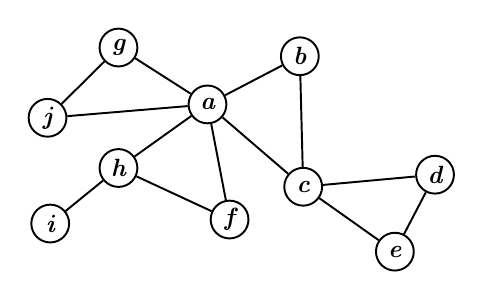
\begin{tikzpicture}[x=0.0085cm,y=-0.0085cm,v/.style={circle,draw,line width=0.7pt,inner sep=0pt,minimum size=0.48cm,font=\small\bfseries\itshape}]
\node[v] (g) at (232,55) {g};
\node[v] (b) at (503,68) {b};
\node[v] (j) at (126,160) {j};
\node[v] (a) at (365,140) {a};
\node[v] (h) at (232,235) {h};
\node[v] (c) at (508,263) {c};
\node[v] (d) at (705,245) {d};
\node[v] (i) at (130,318) {i};
\node[v] (f) at (398,312) {f};
\node[v] (e) at (645,360) {e};
\draw[line width=0.7pt] (g)--(j);
\draw[line width=0.7pt] (g)--(a);
\draw[line width=0.7pt] (j)--(a);
\draw[line width=0.7pt] (a)--(b);
\draw[line width=0.7pt] (b)--(c);
\draw[line width=0.7pt] (a)--(h);
\draw[line width=0.7pt] (a)--(f);
\draw[line width=0.7pt] (a)--(c);
\draw[line width=0.7pt] (h)--(i);
\draw[line width=0.7pt] (h)--(f);
\draw[line width=0.7pt] (c)--(d);
\draw[line width=0.7pt] (c)--(e);
\draw[line width=0.7pt] (d)--(e);
\end{tikzpicture}\\[2pt] Figure 1. The graph $G$ for problem 4\end{center}

\begin{enumerate}[label=(\arabic*)]
\item How many \textit{biconnected components} are in $G$? (3 pts)
\item Please give the \textit{articulation points}. If there is no articulation point, please use $\varnothing$ to denote it. (3 pts)
\item Suppose we are performing a BFS traversal starting with vertex $a$ in alphabetical order. Please show the corresponding BFS-tree. (4 pts)
\end{enumerate}
\end{pastexam}

\begin{pastsoln}
答案：(1) $5$ 個雙連通元件；(2) 割點是 $a$、$c$、$h$；(3) BFS 樹見下圖：$a$ 的子節點是 $b, c, f, g, h, j$，
$c$ 的子節點是 $d, e$，$h$ 的子節點是 $i$。

(1)(2) 是第~23~章，(3) 是第~21~章；放在第~23~章。

\textbf{(1)(2)} 邊有 $13$ 條：$a$--$b$、$a$--$c$、$a$--$f$、$a$--$g$、$a$--$h$、$a$--$j$、$b$--$c$、$c$--$d$、$c$--$e$、$d$--$e$、
$f$--$h$、$g$--$j$、$h$--$i$。 鄰接串列依字母，照資結書虛擬碼~23.4 從 $a$ 開始。 DFS 依序發現
$a, b, c, d, e, f, h, i, g, j$，後向邊是 $\{c, a\}$、$\{e, c\}$、$\{h, a\}$、$\{j, a\}$。

\begin{center}
\small
\setlength{\tabcolsep}{4pt}
\begin{tabular}{ccccc>{\raggedright\arraybackslash}p{0.38\linewidth}}
\toprule
$u$ & $d$ & 子節點 & 後向邊到 & $\mathit{low}$ & 判斷（$v$ 是子節點） \\
\midrule
$a$ & 1 & $b, f, g$ & — & $1$ & 根，三個子節點：割點 \\
$b$ & 2 & $c$ & — & $\min(2, 1) = 1$ & $\mathit{low}[c] = 1 < 2$ \\
$c$ & 3 & $d$ & $a$ & $\min(3, d[a], 3) = 1$ & $\mathit{low}[d] = 3 \ge 3$：割點 \\
$d$ & 4 & $e$ & — & $\min(4, 3) = 3$ & $\mathit{low}[e] = 3 < 4$ \\
$e$ & 5 & — & $c$ & $\min(5, d[c]) = 3$ & 葉節點 \\
$f$ & 6 & $h$ & — & $\min(6, 1) = 1$ & $\mathit{low}[h] = 1 < 6$ \\
$h$ & 7 & $i$ & $a$ & $\min(7, d[a], 8) = 1$ & $\mathit{low}[i] = 8 \ge 7$：割點；$8 > 7$，$\{h, i\}$ 是橋 \\
$i$ & 8 & — & — & $8$ & 葉節點 \\
$g$ & 9 & $j$ & — & $\min(9, 1) = 1$ & $\mathit{low}[j] = 1 < 9$ \\
$j$ & 10 & — & $a$ & $\min(10, d[a]) = 1$ & 葉節點 \\
\bottomrule
\end{tabular}
\end{center}

用邊的堆疊依序彈出五個區塊（虛擬碼第 8 行的條件成立的五次）：
\begin{enumerate}[label=(\roman*)]
\item 從 $d$ 回到 $c$（$\mathit{low}[d] = 3 \ge d[c]$）：$\{c\text{--}d, d\text{--}e, e\text{--}c\}$；
\item 從 $b$ 回到 $a$（$\mathit{low}[b] = 1 \ge d[a]$）：$\{a\text{--}b, b\text{--}c, c\text{--}a\}$；
\item 從 $i$ 回到 $h$（$\mathit{low}[i] = 8 \ge d[h]$）：$\{h\text{--}i\}$；
\item 從 $f$ 回到 $a$：$\{a\text{--}f, f\text{--}h, h\text{--}a\}$；
\item 從 $g$ 回到 $a$：$\{a\text{--}g, g\text{--}j, j\text{--}a\}$。
\end{enumerate}
用頂點寫是 $\{c, d, e\}$、$\{a, b, c\}$、$\{h, i\}$、$\{a, f, h\}$、$\{a, g, j\}$。 割點 $a$ 屬於三個區塊，$c$、$h$
各屬於兩個，和「割點若且唯若屬於兩個以上的區塊」一致（資結書第~23.6~節）。 這張圖沒有孤立頂點，用頂點定
義或邊定義數到的個數一樣，都是 $5$。

\textbf{(3)} 照資結書虛擬碼~21.1，從 $a$ 開始，每個頂點的鄰居依字母順序檢查，第一次看到的頂點才放進
佇列，並以發現它的頂點當父節點。
\begin{center}
\small
\begin{tabular}{clll}
\toprule
取出 & 鄰居（依字母） & 新發現（父節點） & 佇列（左邊是前端） \\
\midrule
$a$ & $b, c, f, g, h, j$ & $b, c, f, g, h, j$（$a$） & $b, c, f, g, h, j$ \\
$b$ & $a, c$ & — & $c, f, g, h, j$ \\
$c$ & $a, b, d, e$ & $d, e$（$c$） & $f, g, h, j, d, e$ \\
$f$ & $a, h$ & — & $g, h, j, d, e$ \\
$g$ & $a, j$ & — & $h, j, d, e$ \\
$h$ & $a, f, i$ & $i$（$h$） & $j, d, e, i$ \\
$j$, $d$, $e$, $i$ & 都已發現 & — & （空） \\
\bottomrule
\end{tabular}
\end{center}
BFS 的順序是 $a, b, c, f, g, h, j, d, e, i$，樹邊有 $9$ 條：$a$--$b$、$a$--$c$、$a$--$f$、$a$--$g$、
$a$--$h$、$a$--$j$、$c$--$d$、$c$--$e$、$h$--$i$。
\begin{center}
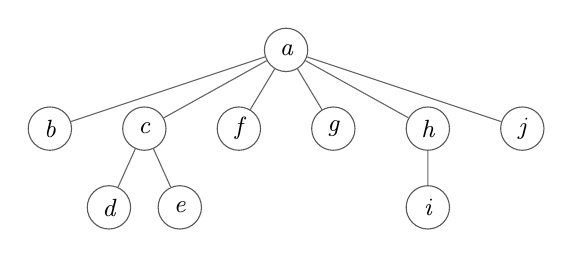
\begin{tikzpicture}[
    tn/.style={circle, draw=black!65, minimum size=0.55cm, inner sep=0pt, font=\small\itshape},
    level distance=10mm, edge from parent/.style={draw=black!60},
    level 1/.style={sibling distance=12mm}, level 2/.style={sibling distance=9mm}]
\node[tn] {a}
    child {node[tn] {b}}
    child {node[tn] {c} child {node[tn] {d}} child {node[tn] {e}}}
    child {node[tn] {f}}
    child {node[tn] {g}}
    child {node[tn] {h} child {node[tn] {i}}}
    child {node[tn] {j}};
\end{tikzpicture}
\end{center}
每個頂點在樹裡的深度就是它到 $a$ 的最短距離（邊數）：$b, c, f, g, h, j$ 是 $1$，$d, e, i$ 是 $2$。
\end{pastsoln}
